
\section{Experiments}

\subsection{SevEval2020}

I use the English task in SemEval2020 benchmark~\cite{semeval2020}.
The corpus is from Clean Corpus of Historical American English (CCOHA)~\cite{ccoha1,ccoha2}, which spans 1810s-2000s.
The corpus is split into two time-specific corpora $C_1, C_2$, as defined in Table~\ref{tab:cchoa}.
There are, in total, 37 target words, and I will evaluate the proposed method in both binary classification and ranking problems.



\noindent\textbf{Metrics.} 
For classification, we use standard accuracy. For the ranking problem, we use spearman's correlation.

\begin{table}[th]
\centering
\resizebox{0.8\linewidth}{!}{%
\begin{tabular}{@{}crrrr@{}}
\toprule
\multicolumn{1}{r}{} & \multicolumn{1}{c}{periods} & \multicolumn{1}{c}{tokens} & \multicolumn{1}{c}{types} & \multicolumn{1}{c}{TTR} \\ \midrule
\multicolumn{1}{c|}{$C_1$} & 1810–1860 & 6.5M & 87k & 13.38 \\
\multicolumn{1}{c|}{$C_2$} & 1960-2010 & 6.7M & 150k & 22.38 \\ \bottomrule
\end{tabular}%
}
\caption{Statistics of test corpora. TTR = Type-Token ratio (number of types / number of tokens * 1000)}
\label{tab:cchoa}
\end{table}

%\AL{scale of data, where does the data come from, how do they obtain the ground truth, what are the sub-tasks, evaluation metrics}

\subsection{Implementation Details}\label{sec:impl_details}
For the empirical minimizer, we use a modified BERT~\cite{BERT} model.
In my case, I do not necessarily need a model to achieve the SOTA language modeling performance. 
To make the training less computationally intensive, I decrease the hidden units from 768 to 128, 12 attention heads to 8 attention heads, and set the max length to 128.
The modification reduces the model size from 110M to 10M parameters.
To approximate the hessian inverse product in Eq.~\ref{eq:scores_mlm}, we set the scale to be 5000, recursion depth 10000, and damping $1e-2$.
The source code is released at https://github.com/andrewliao11/csc2611-course-semantic-change.



\begin{figure*}[t]
\centering
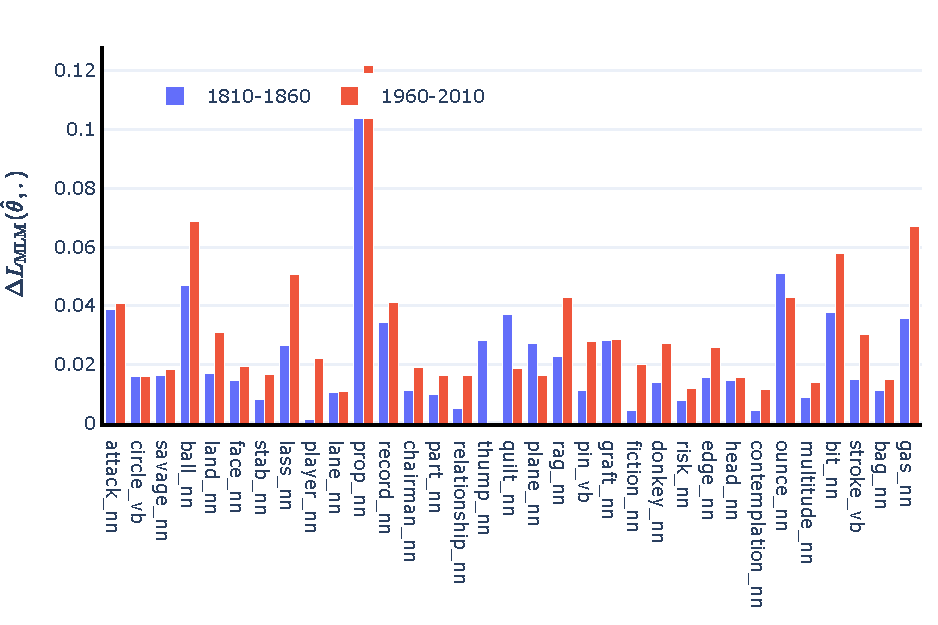
\includegraphics[width=0.8\textwidth]{../project/src/scale_5000-recursion_depth_10000/influences_by_corpus.pdf}
\caption{\textbf{Predicted Influences in different time periods.}}
\label{fig:inf_time}
\end{figure*}

\subsection{Binary Classificaiton}

For binary classification, I achieve 0.7 accuracies, outperforming 20 out of 22 participants in SemEval challenge~\cite{semeval2020}.
Since each team can submit ten trials in the challenge, I try ten different thresholds that equally split the range between maximum influence and min influence and report the best performance.
I show the predicted influences in Fig.~\ref{fig:binary}.
For the words that do not experience any LSC change, the word ``ball'' has the greatest predicted influence. 
From the ground truth rank, the word ``ball'' is the 5th highest word, with a score of $0.409$.
The binary classification considers if the target word gain or loss any sense between two corpora, which is different from how the ground truth of the rank is measured.
%I will discuss the comparison between binary classification and ranking problem in Sec.~\ref{sec:}




\subsection{Ranking}


For the ranking problem, I achieve $0.59$ spearman's correlation, outperforming all 22 participants in SemEval2020~\cite{semeval2020}.
The predicted influences and the ground truth grades are shown in Fig.~\ref{fig:rank}.
One failure case is the word ``plane'', which has a ground truth grade of 0.88, while the predicted influence is as low as 0.02, which ranks middle (19th) in terms of predicted influence.



\begin{figure}[t]
\centering
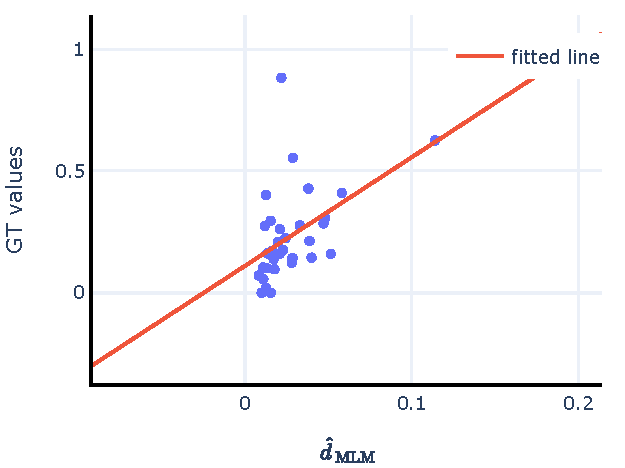
\includegraphics[width=0.5\textwidth]{../project/src/scale_5000-recursion_depth_10000/influences_grade_scatter.pdf}
\caption{\textbf{Predicted Influences vs. ground truth grade.}}
\label{fig:rank}
\end{figure}


\begin{figure*}[t]
\centering
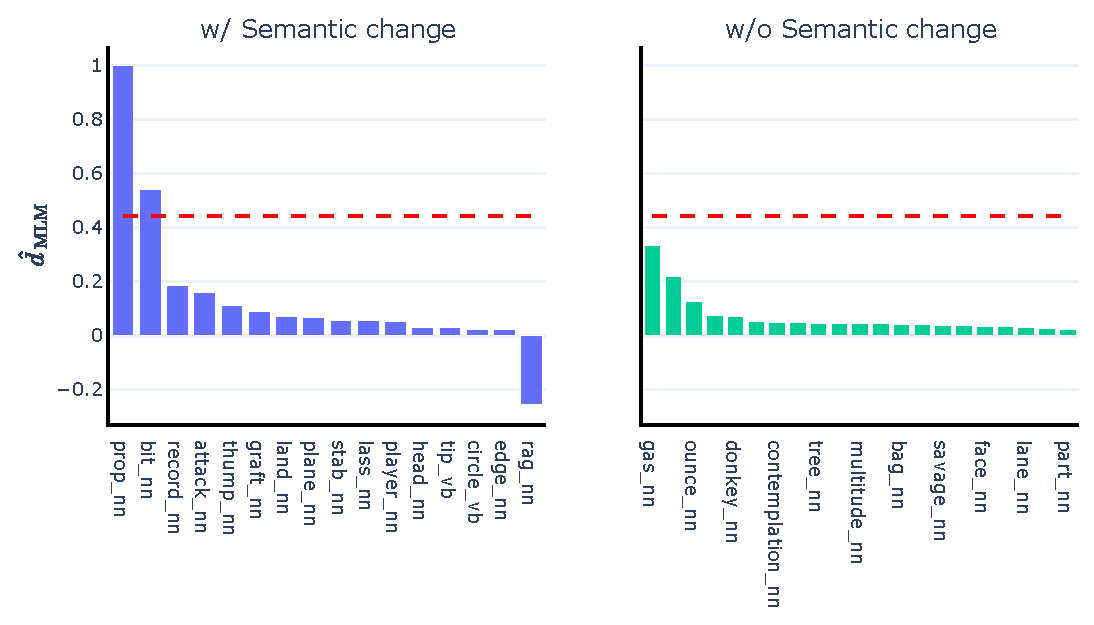
\includegraphics[width=0.8\textwidth]{../project/src/scale_1000-recursion_depth_1000/influences_binary.pdf}
\caption{\textbf{$R_{1000, 1000}$: Predicted Influences in different time periods.} The red dash lines are the threshold for binary classification.}
\label{fig:inf_binary_r_1000_1000}
\end{figure*}


%\subsection{Qualitative Results}

\subsection{Analysis}

\subsubsection{Qualitative Analysis}
The estimated LSC scores are the average predicted influences. 
In Fig.~\ref{fig:inf_time}, I show the predicted influences in $C_1$ and $C_2$. 
The word ``player'', ``fiction'', and ``relationship'' have the most difference between predicted influences in $C_1$ and $C_2$, more than 300\%.
For certain words, the computation of inverse HVP diverges. In these cases, I treat them as an outlier and do not consider their values.


\subsubsection{Hyperparameter Analysis}
To compute the influence functions, we adopt the approximation approach~\cite{second-order-approx}, which includes several hyperparameters.
When performing the approximation, two hyperparameters govern the stability of the approximation, scale and recursion depth. 
As mentioned in Sec.~\ref{sec:impl_details}, we set them to be $(5000, 10000)$, denoted as $R_{5000, 10000}$.
In this section, we show other two configurations $R_{1000, 1000}$ and $R_{1000, 10000}$.
The comparison of three different configurations in binary classification and the ranking problem is shown in Table.~\ref{tab:hyperparams}.
Both the performances of binary classification and the ranking problem vary a lot.
The binary classification results in $R_{1000, 1000}$ might look nice, achieving 62\% accuracy, outperforming 14 out of 22 teams in the SemEval2020 challenges.
However, from Fig.~\ref{fig:inf_binary_r_1000_1000} and Fig.~\ref{fig:inf_scatter_r_1000_1000}, there are only two positive predictions and all the other are predicted negative. 

From the hyperparameters analysis results, the proposed approach requires lots of tuning to get great results.


\begin{table}[t]
\centering
\resizebox{\linewidth}{!}{%
\begin{tabular}{@{}rcc@{}}
\toprule
 & \multicolumn{1}{r}{Binary Classification} & \multicolumn{1}{r}{Ranking Problem} \\ \midrule
\multicolumn{1}{r|}{$R_{5000, 10000}$} & \textbf{0.7} & \textbf{0.59} \\
\multicolumn{1}{r|}{$R_{1000, 10000}$} & 0.37 & 0.57 \\
\multicolumn{1}{r|}{$R_{1000, 1000}$} & 0.62 & 0.27 \\ \bottomrule
\end{tabular}%
}
\caption{\textbf{Comparison between different hyperparameters configurations.}}
\label{tab:hyperparams}
\end{table}





\begin{figure}[t]
\centering
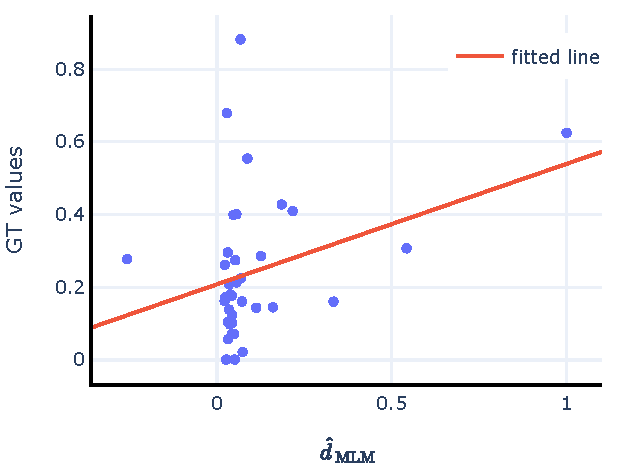
\includegraphics[width=0.5\textwidth]{../project/src/scale_1000-recursion_depth_1000/influences_grade_scatter.pdf}
\caption{\textbf{$R_{1000, 1000}$: Predicted Influences vs. ground truth grade.}}
\label{fig:inf_scatter_r_1000_1000}
\end{figure}